\documentclass{book}
\usepackage{amsmath}
\usepackage{bm}
\usepackage{colortbl}
\usepackage{graphicx}
\usepackage{caption}
\usepackage{fullpage}
\usepackage{afterpage}
\usepackage{multirow}
\usepackage[nodisplayskipstretch]{setspace}
\usepackage{booktabs}
\usepackage{gensymb}
\usepackage{parskip}
\usepackage{xr}
\usepackage{pdflscape}
\usepackage[inline]{enumitem}
\usepackage{wrapfig}
\usepackage{longtable}
\usepackage{subfig}
\usepackage[natbib=true,subentry,backend=biber,sorting=none,citestyle=authoryear-comp]{biblatex}
\addbibresource{citation/Thesis.bib}
\usepackage[hidelinks]{hyperref}
\usepackage{geometry}
\geometry{
	top=1in,            % <-- you want to adjust this
	inner=1in,
	outer=1in,
	bottom=1in,
	headheight=3ex,       % <-- and this
	headsep=2ex,          % <-- and this
}
\usepackage{fancyhdr}
\usepackage{fixltx2e}
\usepackage[acronym,nomain,toc,makeindex ]{glossaries}
\usepackage{cleveref} %This need to be the last package for it to work properly 


\pagestyle{fancy}

\title{Genetic and Environmental risk factors of Schizophrenia and Autism}
\date{\today}
\author{\href{mailto:choishingwan@gmail.com}{Choi Shing Wan}\\
	
\includegraphics[width=0.5\textwidth]{hkuLogo.jpg}}
\singlespacing
\renewcommand*\contentsname{Contents}
\onehalfspacing
%\doublespacing

%\includeonly{environmental_risk/er_chapter,supplementary_materials}

\makeglossary
\newacronym{SCZ}{SCZ}{Schizophrenia}
\newacronym{ASD}{ASD}{Autism Spectrum Disorder}
\newacronym[longplural={Genome Wide Association Studies}]{GWAS}{GWAS}{Genome Wide Association Study}
\newacronym{wgs}{WGS}{Whole Genome Sequencing}
\newacronym{SNP}{SNP}{Single Nucleotide Polymorphism}
\newacronym{LD}{LD}{Linkage Disequilibrium}
\newacronym{PGS}{PGS}{Polygenic Risk Score}
\newacronym{tSVD}{tSVD}{Truncated Singular Value Decomposition}
\newacronym{SVD}{SVD}{Singular Value Decomposition}
\newacronym{shrek}{\textit{SHREK}}{SNP Heritability and Risk Estimation Kit}
\newacronym{gcta}{\textit{GCTA}}{Genome-wide Complex Trait Analysis}
\newacronym{ldsc}{\textit{LDSC}}{LD SCore}
\newacronym{CEU}{CEU}{Northern Europeans from Utah}
\newacronym{se}{SE}{Standard Error}
\newacronym{maf}{maf}{Minor Allele Frequency}
\raggedbottom %Remove it before printing as this is something to do with global settings. Can make each page look uneven but more dense. 
\makeindex
\begin{document}\thispagestyle{empty}
\pagestyle{empty}

%\maketitle
\begin{titlepage}
	\begin{center}
		\vspace*{1cm}
		
		\Huge
		\textbf{Heritability Estimation and Risk Prediction in Schizophrenia}
		
		\vspace{0.5cm}
		\LARGE
		
		\vspace{1.5cm}
		
		\textbf{\href{mailto:choishingwan@gmail.com}{Choi Shing Wan}}
		
		\vfill
		
		A thesis submitted in partial fulfillment of the requirements for \\
		the Degree of Doctor of Philosophy
		
		\vspace{0.8cm}
		
		
\includegraphics[width=0.4\textwidth]{figure/hkuLogo.jpg}
		
		\Large
		Department of Psychiatry\\
		University of Hong Kong\\
		Hong Kong\\
		\today
		
	\end{center}
\end{titlepage}


\frontmatter 

	\cleardoublepage
	\phantomsection
	\addcontentsline{toc}{chapter}{Declaration}
	\chapter*{Declaration}
	\cleardoublepage
	\phantomsection
	\addcontentsline{toc}{chapter}{Acknowledgments}
	\chapter*{Acknowledgements}
	\cleardoublepage
	\phantomsection
	\begin{singlespace}
	\printglossary[title=Abbreviations,toctitle=Abbreviations]
	\cleardoublepage
	\phantomsection
	%To generate the correct abbreviations, use alt+shift+F1 twice before using F1
	
	\cleardoublepage
	\phantomsection
	\addcontentsline{toc}{chapter}{Contents}
		\tableofcontents
		\listoffigures
	\end{singlespace}
\mainmatter
	\chapter*{Introduction}
		\addcontentsline{toc}{chapter}{Introduction}
	\pagestyle{fancy}
	\chapter*{Some considerations}
	\begin{enumerate}
		\item PRSice requires the phenotype to aid its selection (More information= stronger)
		\item It seems like LDSC doesn't necessary perform badly in oligogenic situation.
		Rather, it is that when the trait is oligogenic, it is more likely for LDSC to behaviour in a strange way.
		\item For each condition: extreme phenotype, quantitative trait, case control, we can have a separated review. 
		Discuss on the benefits and challenges of each condition and the method we deal with them.
		So we can have two chapters (case control, quantitative trait) where extreme phenotype can be a big subsection within quantitative trait.
		\item For each chapter, there will be this introduction (review on the method), our methodology (Calculation, implementation and also simulation), result (the simulation result). 
		Then we can have the application (PGC, network)
	\end{enumerate}
	
	\chapter{Literature Review}
	\section{Twin Studies}
	Should briefly talk about how Twin modeling was used for finding the GE contribution.
	Should also mention the ACE model.
	At the end, we can talk about the heritability estimates of SCZ and AD
	\section{Searching for Genetic Variants}
	\subsection{Role of Common Variants}
	\subsubsection{Genome Wide Association Study}
	Should talk about what is GWAS and how it is used.
	Should also talk about the current GWAS studies in SCZ and AD
	\subsection{Role of Rare Variants}
	\subsubsection{Exome Sequencing}
	Similar to the GWAS.
	Talk about the Pros and Cons.
	Need to briefly mention the Denovo paper and Shaun's paper.					
	\subsubsection{Whole Genome Sequencing}
	Very very brief description of WGS and the current status.
	\section{Narrow Sense Heritability}
	\section{Risk Prediction}
	\section{Summary}
	
	\chapter{Heritability Estimation}
	\section{Introduction}
	\section{Methodology}	
		The overall aims of this study is to develop a robust algorithm for the estimation of the narrow sense heritability using only the summary statistic from a \gls{GWAS} study. The work in this chapter were done in collaboration with my colleagues who have kindly provide their support and knowledges to make this piece of work possible.
		Dr Johnny Kwan, Dr Miaxin Li and Professor Sham have helped to laid the framework of this study. Dr Timothy Mak has derived the mathematical proof for our heritability estimation method. Miss Yiming Li, Dr Johnny Kwan, Dr Miaxin Li, Dr Timothy Mak and Professor Sham have helped with the derivation of the standard error of the heritability estimation. Dr Henry Leung has provided critical suggestions on the implementation of the algorithm.
		\subsection{Heritability Estimation}
			The narrow-sense heritability is defined as 
			$$
				h^2 = \frac{\mathrm{Var}(X)}{\mathrm{Var}(Y)}
			$$
			where $\mathrm{Var}(X)$ is the variance of the genotype and $\mathrm{Var}r(Y)$ is the variance of the phenotype.
			In a \gls{GWAS}, regression were performed between the \glspl{SNP} and the phenotypes, giving
			\begin{equation}
				Y=\beta X+\epsilon
				\label{eq:standardRegress}
			\end{equation}
			where $Y$ and $X$ are the standardized phenotype and genotype respectively. 
			$\epsilon$ is then the error term, accounting for the non-genetic elements contributing to the phenotype (e.g. Environment factors).
			Based on \cref{eq:standardRegress}, one can then have
			\begin{align}
				\mathrm{Var}(Y) = \mathrm{Var}(\beta X)+ \mathrm{Var}(\epsilon) \nonumber\\
				\mathrm{Var}(Y) = \beta^\mathrm{Var}(X) \nonumber\\
				\beta^2\frac{\mathrm{Var}(X)}{\mathrm{Var}(Y)}= 1
				\label{eq:betaHeri}
			\end{align}
			$\beta^2$ is then considered as the portion of phenotype variance explained by the variance of genotype, which can also be considered as the narrow-sense heritability of the phenotype.
					
			A challenge in calculating the heritability from \gls{GWAS} data is that usually only the test-statistic or p-value were provided and one will not be able to directly calculate the heritability based on \cref{eq:betaHeri}. In order to estimation the heritability of a trait from the \gls{GWAS} test-statistic, we first observed that when both $X$ and $Y$ are standardized, $\beta^2$ will be equal to the coefficient of determination ($r^2$). Then, based on properties of the Pearson product-moment correlation coefficient:
			\begin{equation}
				r = \frac{t}{\sqrt{n-2+t^2}}
				\label{eq:pearsonProduct}
			\end{equation}
			where $t$ follows the student-t distribution and $n$ is the number of samples.
			One can then obtain the $r^2$ by taking the square of \cref{eq:pearsonProduct}
			\begin{equation}
				r^2 = \frac{t^2}{n-2+t^2}
				\label{eq:oriRSquared}
			\end{equation}
			It is observed that $t^2$ will follow the F-distribution and when $n$ is big, $t^2$ will converge into $\chi^2$ distribution.
			
			When the effect size is small and $n$ is big, $r^2$ will be approximately $\chi^2$ distributed with mean $\sim 1$. 
			We can then approximate \cref{eq:oriRSquared} as
			\begin{equation}
				r^2= \frac{\chi^2}{n}
				\label{eq:approxChi}
			\end{equation}
			and define the \emph{observed} effect size of each \gls{SNP} to be
			\begin{equation}
			f=\frac{\chi^2-1}{n}
			\label{eq:observedEffect}
			\end{equation}
			
			When there are \gls{LD} between each individual \glspl{SNP}, the situation will become more complicated as each \glspl{SNP}' observed effect will contains effect coming from other \glspl{SNP} in \gls{LD} with it. 
			\begin{equation}
			f_{observed} = f_{true}+f_{LD}
			\label{eq:conceptF}
			\end{equation}
			
			To account for the \gls{LD} structure, we first assume our phenotype $\boldsymbol{Y}$ and genotype $\boldsymbol{X}=(X_1,X_2,\dots,X_m)^t$ are standardized and that
			\begin{align*}
				\boldsymbol{Y}\sim f(0,1) \\
				\boldsymbol{X}\sim f(0,\boldsymbol{R})
			\end{align*}
			Where $\boldsymbol{R}$ is the \gls{LD} matrix between \glspl{SNP}.
			
			We can then express \cref{eq:standardRegress} in matrix form:
			\begin{align}
				\boldsymbol{Y}=\boldsymbol{\beta}^t\boldsymbol{X}+\epsilon
				\label{eq:matrixRegress}
			\end{align}
			Definition of heritability will then become
			\begin{align}
				Heritability& = \frac{\mathrm{Var}(\boldsymbol{\beta}^t\boldsymbol{X})}{\mathrm{Var}(\boldsymbol{Y})} \nonumber\\
				&=\mathrm{Var}(\boldsymbol{\beta}^t\boldsymbol{X})
			\end{align}
			If we then assume now that $\boldsymbol{\beta} = (\beta_1, \beta_2,\dots,\beta_m)^t$ has distribution
			\begin{align*}
				\boldsymbol{\beta}&\sim f(0,\boldmath{H})\\
				\boldsymbol{H}&=diag(\boldsymbol{h})\\
				\boldsymbol{h}&=(h_1^2,h_2^2,\dots,h_m^2)^t
			\end{align*}
			where $\boldsymbol{H}$ is the variance of the true effect. 
			It is shown that heritability can be expressed as %The later part was gone because that will contains E(\beta) which = 0
			\begin{align}
			\mathrm{Var}(\boldsymbol{\beta}^t\boldsymbol{X}) &= \mathrm{E}_X\mathrm{Var}_{\beta|X}(\boldsymbol{X}^t\boldsymbol{\beta})+\mathrm{Var}_X\mathrm{E}_{(\beta|X)}(\boldsymbol{\beta}^2\boldsymbol{X}) \nonumber\\
			&=\mathrm{E}_X(\boldsymbol{X}^t\boldsymbol{\beta\beta}^T\boldsymbol{X}) \nonumber\\ 
			&= \mathrm{E}_X(\boldsymbol{X}^t\boldsymbol{HX}) \nonumber\\
			&= \mathrm{E}(\boldsymbol{X})^t\boldsymbol{H}\mathrm{E}(\boldsymbol{X})+\mathrm{Tr}(\mathrm{Var}(\boldsymbol{X}\boldsymbol{H})) \nonumber\\
			&=\mathrm{Tr}(\mathrm{Var}(\boldsymbol{X}\boldsymbol{H})) \nonumber\\
			&=\sum_ih_i^2
			\label{eq:proveHerit}
			\end{align}
			
			Now if we consider the covariance between \gls{SNP} i ($X_i$) and $Y$, we have
			\begin{align}
			 \mathrm{Cov}(\boldsymbol{X}_i,\boldsymbol{Y}) &= \mathrm{Cov}(\boldsymbol{X}_i,\boldsymbol{\beta}^t\boldsymbol{X}+\epsilon) \nonumber\\
			 &=\mathrm{Cov}(\boldsymbol{X}_i,\boldsymbol{\beta}^t\boldsymbol{X}) \nonumber\\
			 &=\sum_j{\mathrm{Cov}(\boldsymbol{X}_i,\boldsymbol{X}_j)\boldsymbol{\beta}_j} \nonumber\\
			 &=\boldsymbol{R}_i\boldsymbol{\beta}_j
			 \label{eq:covPhenoTrue}
			\end{align}
			As both $X$ and $Y$ are standardized, the covariance will equal to the correlation and we can define the correlation between \gls{SNP} i and $Y$ as
			\begin{equation}
				\rho_i = \boldsymbol{R}_i\boldsymbol{\beta}_j
				\label{eq:corPhenoTrue}
			\end{equation}
			In reality, the \emph{observed} correlation usually contains error. 
			Therefore we define the \emph{observed} correlation to be
			\begin{equation}
			\hat{\rho_i} = \rho_i+\frac{\epsilon_i}{\sqrt{n}}
			\label{eq:obsPheno}
			\end{equation}
			for some error $\epsilon_i$. 
			The distribution of the correlation coefficient about the true correlation $\rho$ is approximately
			$$
				\hat{\rho_i}\sim f(\rho_i, \frac{(1-\rho^2)^2}{n})
			$$
			By making the assumption that $\rho_i$ is close to 0 for all $i$, we have 
			\begin{align*}
				\mathrm{E}(\epsilon_i|\rho_i)&\sim 0\\
				\mathrm{Var}(\epsilon_i|\rho_i)&\sim 1
			\end{align*}
			We then define our $z$-statistic and $\chi^2$-statistic as
			\begin{align*}
				z_i &= \hat{\rho_i}\sqrt{n} \\
				\chi^2 &= z_i^2\\
				&=\hat{\rho_i}^2n
			\end{align*}
			From \cref{eq:obsPheno} and \cref{eq:corPhenoTrue}, $\chi^2$ can then be expressed as
			\begin{align*}
			\chi^2&=\hat{\rho}^2n\\
			&=n(\boldsymbol{R}_i\boldsymbol{\beta}_j+\frac{\epsilon_i}{\sqrt{n}})^2
			\end{align*}
			The expectation of $\chi^2$ is then
			\begin{align*}
			\mathrm{E}(\chi^2) &= n(\boldsymbol{R}_i\boldsymbol{\beta\beta}^t\boldsymbol{R}_i+2\boldsymbol{R}_i\boldsymbol{\beta}\frac{\epsilon_i}{\sqrt{n}}+\frac{\epsilon_i^2}{n}) \\
			&= n\boldsymbol{R}_i\boldsymbol{H}\boldsymbol{R}_i+1
			\end{align*}
			To derive least square estimates of $h_i^2$, we need to find $\hat{h_i^2}$ which minimizes
			\begin{align*}
				\sum_i(\chi_i^2-\mathrm{E}(\chi_i^2))^2&=\sum_i(\chi_i^2-(n\boldsymbol{R}_i\boldsymbol{H}\boldsymbol{R}_i+1))^2 \\
				&=\sum_i(\chi_i^2-1-n\boldsymbol{R}_i\boldsymbol{H}\boldsymbol{R}_i)^2 
			\end{align*}
			If we define 
			\begin{equation}
			f_i= \frac{\chi_i^2-1}{n}
			\label{eq:defineF}
			\end{equation}
			we got
			\begin{align}
			\sum_i(\chi_i^2-\mathrm{E}(\chi_i^2))^2&=\sum_i(f_i-\boldsymbol{R}_i\boldsymbol{H}\boldsymbol{R}_i)^2 \nonumber\\
			&=\boldsymbol{ff}^t-2\boldsymbol{f}^t\boldsymbol{R_{sq}\hat{h}}+\boldsymbol{\hat{h}}^t\boldsymbol{R_{sq}}^t\boldsymbol{R_{sq}\hat{h}}
			\label{eq:leastSquareH}
			\end{align}
			where $\boldsymbol{R_{sq}} = \boldsymbol{R}\circ\boldsymbol{R}$.
			By differentiating \cref{eq:leastSquareH} w.r.t $\hat{h}$ and set to 0, we get
			\begin{align}
				2\boldsymbol{R_{sq}}^t\boldsymbol{R_{sq}}\boldsymbol{\hat{h^2}}-2\boldsymbol{R_{sq}f}&=0 \nonumber\\
				\boldsymbol{R_{sq}}\boldsymbol{\hat{h^2}} &=\boldsymbol{f}
				\label{eq:shrekEq}
			\end{align}
			And the heritability is then defined as 
			\begin{equation}
			\hat{Heritability} = \boldsymbol{1}^t\boldsymbol{R_{sq}}^{-1}\boldsymbol{f}
			\label{eq:fullShrek}
			\end{equation}
		\subsection{Calculating the \glsentrylong{se}}
			From \cref{eq:fullShrek}, we can derive the variance of heritability $H$ as 
			\begin{align}
				\mathrm{Var}(H) &= \mathrm{E}[H^2]-\mathrm{E}[H]^2\nonumber\\
				&=\mathrm{E}[(\boldsymbol{1}^t\boldsymbol{R_{sq}}^{-1}\boldsymbol{f})^2]-\mathrm{E}[\boldsymbol{1}^t\boldsymbol{R_{sq}}^{-1}\boldsymbol{f}](\mathrm{E}[\boldsymbol{1}^t\boldsymbol{R_{sq}}^{-1}\boldsymbol{f}])^t \nonumber \\
				&=\mathrm{E}[\boldsymbol{1}^t\boldsymbol{R_{sq}}^{-1}\boldsymbol{ff}^t\boldsymbol{R_{sq}}^{-1}\boldsymbol{1}]-\mathrm{E}[\boldsymbol{1}^t\boldsymbol{R_{sq}}^{-1}\boldsymbol{f}](\mathrm{E}[\boldsymbol{1}^t\boldsymbol{R_{sq}}^{-1}\boldsymbol{f}])^t \nonumber \\
				&=\boldsymbol{1}^t\boldsymbol{R_{sq}}^{-1}\mathrm{E}[\boldsymbol{ff}^t]\boldsymbol{R_{sq}}^{-1}\boldsymbol{1}-\mathrm{E}[\boldsymbol{1}^t\boldsymbol{R_{sq}}^{-1}\boldsymbol{f}](\mathrm{E}[\boldsymbol{1}^t\boldsymbol{R_{sq}}^{-1}\boldsymbol{f}])^t \nonumber \\
				&=\boldsymbol{1}^t\boldsymbol{R_{sq}}^{-1}\mathrm{Var}(\boldsymbol{f})\boldsymbol{R_{sq}}^{-1}\boldsymbol{1}+\mathrm{E}[\boldsymbol{1}^t\boldsymbol{R_{sq}}^{-1}\boldsymbol{f}](\mathrm{E}[\boldsymbol{1}^t\boldsymbol{R_{sq}}^{-1}\boldsymbol{f}])^t-\mathrm{E}[\boldsymbol{1}^t\boldsymbol{R_{sq}}^{-1}\boldsymbol{f}](\mathrm{E}[\boldsymbol{1}^t\boldsymbol{R_{sq}}^{-1}\boldsymbol{f}])^t \nonumber\\
				&=\boldsymbol{1}^t\boldsymbol{R_{sq}}^{-1}\mathrm{Var}(\boldsymbol{f})\boldsymbol{R_{sq}}^{-1}\boldsymbol{1}
				\label{eq:varHvarf}
			\end{align}
			Therefore, to obtain the variance of $H$, we first need to calculate the variance covariance matrix of $\boldsymbol{f}$.
			
			We first consider the standardized genotype $X_i$ with standard normal mean $z_i$ and non-centrality parameter
			$\mu_i$, we have
			\begin{align*}
				\mathrm{E}[X_i]&=\mathrm{E}[z_i+\mu_i]\\
				&=\mu_i\\
				\mathrm{Var}(X_i) &=\mathrm{E}[(z_i+\mu_i)^2]+\mathrm{E}[(z_i+\mu_i)]^2\\
				&=\mathrm{E}[z_i^2+\mu_i^2+2z_i\mu_i]+\mu_i^2\\
				&=1 \\
				\mathrm{Cov}(X_i,X_j)&=\mathrm{E}[(z_i+\mu_i)(z_j+\mu_j)]-\mathrm{E}[z_i+\mu_i]\mathrm{E}[z_j+\mu_j]\\
				&=\mathrm{E}[z_iz_j+z_i\mu_j+\mu_iz_j+\mu_i\mu_j]-\mu_i\mu_j\\
				&=\mathrm{E}[z_iz_j]+\mathrm{E}[z_i\mu_j]+\mathrm{E}[z_j\mu_i]+\mathrm{E}[\mu_i\mu_j]-\mu_i\mu_j\\
				&=\mathrm{E}[z_iz_j]
			\end{align*}
			As the genotypes are standardized, therefore $\mathrm{Cov}(X_i,X_j)==\mathrm{Cor}(X_i,X_j)$, we can obtain
			$$
				\mathrm{Cov}(X_i,X_j)=\mathrm{E}[z_iz_j]=R_{ij}
			$$
			where $R_{ij}$ is the \gls{LD} between \gls{SNP}$_i$ and \gls{SNP}$_j$.
			Given these information, we can then calculate $\mathrm{Cov}(\chi_i^2,\chi_j^2)$ as:
			\begin{align*}
				\mathrm{Cov}(X_i^2,X_j^2)&=\mathrm{E}[(z_i+\mu_i)^2(z_j+\mu_j)^2]-\mathrm{E}[z_i+\mu_i]\mathrm{E}[z_j+\mu_j]\\
				&=\mathrm{E}[(z_i^2+\mu_i^2+2z_i\mu_i)(z_j^2+\mu_j^2+2z_j\mu_j)]-\mathrm{E}[z_i^2+\mu_i^2+2z_i\mu_i]\mathrm{E}[z_j^2+\mu_j^2+2z_j\mu_j]\\
				&=\mathrm{E}[(z_i^2+\mu_i^2+2z_i\mu_i)(z_j^2+\mu_j^2+2z_j\mu_j)]-(\mathrm{E}[z_i^2]+\mathrm{E}[\mu_i^2]+2\mathrm{E}[z_i\mu_i])(\mathrm{E}[z_j^2]+\mathrm{E}[\mu_j^2]+2\mathrm{E}[z_j\mu_j])\\
				&=\mathrm{E}[z_i^2(z_j^2+\mu_j^2+2z_j\mu_j)+\mu_i^2(z_j^2+\mu_j^2+2z_j\mu_j)+2z_i\mu_i(z_j^2+\mu_j^2+2z_j\mu_j)]-(1+\mu_i^2)(1+\mu_j^2)\\
				&=\mathrm{E}[z_i^2(z_j^2+\mu_j^2+2z_j\mu_j)]+\mu_i^2\mathrm{E}[z_j^2+\mu_j^2+2z_j\mu_j]+2\mu_i\mathrm{E}[z_i(z_j^2+\mu_j^2+2z_j\mu_j)]-(1+\mu_i^2)(1+\mu_j^2)\\
				&=\mathrm{E}[z_i^2z_j^2+z_i^2\mu_j^2+2z_i^2z_j\mu_j]+\mu_i^2+\mu_i^2\mu_j^2+2\mu_i\mathrm{E}[z_iz_j^2+z_i\mu_j^2+2z_iz_j\mu_j]-(1+\mu_i^2)(1+\mu_j^2)\\
				&=\mathrm{E}[z_i^2z_j^2]+\mu_j^2+\mu_i^2+\mu_i^2\mu_j^2+4\mu_i\mu_j\mathrm{E}[z_iz_j]-(1+\mu_i^2+\mu_j^2+\mu_i\mu_j)\\
				&=\mathrm{E}[z_i^2z_j^2]+4\mu_i\mu_j\mathrm{E}[z_iz_j]-1
			\end{align*}
			Remember that $\mathrm{E}[z_iz_j] = R_{ij}$, we then have
			$$
				\mathrm{Cov}(X_i^2, X_j^2)=\mathrm{E}[z_i^2z_j^2]+4\mu_i\mu_jR_{ij}-1
			$$
			By definition, 
			$$
				z_i|z_j\sim N(\mu_i+R_{ij}(z_j-\mu_j),1-R_{ij}^2)
			$$
			We can then calculate $\mathrm{E}[z_i^2z_j^2]$ as
			\begin{align*}
				\mathrm{E}[z_i^2z_j^2]&=\mathrm{Var}[z_iz_j]+\mathrm{E}[z_iz_j]^2\\
				&=\mathrm{E}[\mathrm{Var}(z_iz_j|z_i)]+\mathrm{Var}[\mathrm{E}[z_iz_j|z_i]]+R_{ij}^2\\
				&=\mathrm{E}[z_j^2\mathrm{Var}(z_i|z_j)]+\mathrm{Var}[z_j\mathrm{E}[z_i|z_j]]+R_{ij}^2\\
				&=(1-R_{ij}^2)\mathrm{E}[z_j^2]+\mathrm{Var}(z_j(\mu_i+R_{ij}(z_j-\mu_j)))+R_{ij}^2\\
				&=(1-R_{ij}^2)+\mathrm{Var}(z_j\mu_i+R_{ij}z_j^2-\mu_jz_jR_{ij})+R_{ij}^2\\
				&=1+\mu_i^2\mathrm{Var}(z_j)+R_{ij}^2\mathrm{Var}(z_j^2)-\mu_j^2R_{ij}^2\mathrm{Var}(z_j)\\
				&=1+2R_{ij}^2
			\end{align*}
			As a result, the variance covariance matrix of the $\chi^2$ variances represented as
			\begin{equation}
				\mathrm{Cov}(X_i^2,X_j^2) = 2R_{ij}^2+4R_{ij}\mu_i\mu_j
				\label{eq:finalChi}
			\end{equation}
			Considering that we only have the \emph{observed} expectation, we should re-define \cref{eq:finalChi} as
			\begin{equation}
				\mathrm{Cov}(X_i^2,X_j^2) = \frac{2R_{ij}^2+4R_{ij}\mu_i\mu_j}{n^2}
				\label{eq:finalChiCov}
			\end{equation}
			where $n$ is the sample size.
			
			By substituting \cref{eq:finalChiCov} into \cref{eq:varHvarf}, we will get
			\begin{align}
				\mathrm{Var}(H) &=\boldsymbol{1}^t\boldsymbol{R_{sq}}^{-1}\frac{2\boldsymbol{R_{sq}}+4\boldsymbol{R}\circ \boldsymbol{zz}^t}{n^2}\boldsymbol{R_{sq}}^{-1}\boldsymbol{1}
				\label{eq:covH}
			\end{align}
			where $\boldsymbol{z} = \sqrt{\boldsymbol{\chi^2}}$ from \cref{eq:defineF}, with the direction of effect as its sign and $\circ$ is the element-wise product (Hadamard product).
			 
			Problem with \cref{eq:covH} were that not only does it requires the direction of effect, the error in the \gls{LD} matrix also tends to amplify due to its predominant role in the equation, leading to un-stable estimation of the \gls{se}.
			 
			Another way to get the \gls{se} is based on the fact that $\boldsymbol{f}$ is approximately $\chi^2$ distributed. 
			Therefore \cref{eq:shrekEq} can be viewed as a decomposition of a vector of $\chi^2$ distributions with degree of freedom of 1. 
			Replacing the vector $\boldsymbol{f}$ with a vector of 1, we can perform the decomposition of the degree of freedom, getting the ``effective number''($e$) of the association\citep{Li2011b}. 
			Substituting $e$ into the variance equation of non-central $\chi^2$ distribution will yield
			\begin{equation}
			\mathrm{Var}(H) = \frac{2(e+2H)}{n^2}
			\label{eq:effectiveChi}
			\end{equation}
			 \cref{eq:effectiveChi} will gives us an heuristic estimation of the \gls{se}. 
		\subsection{Calculating the \glsentrylong{LD} matrix}
			To estimate the heritability, the population \gls{LD} matrix is required.
			In reality, one can only obtain the \gls{LD} matrix based on a subset of the population (e.g. the 1000 genome project\parencite{Project2012} or the HapMap project\parencite{Altshuler2010}).
			There are therefore sampling errors among the \gls{LD} elements. 
			
			Now if we consider \cref{eq:fullShrek}, the $\boldsymbol{R_{sq}}$ matrix is required.
			As the squared \gls{LD} is used, a positive bias is induced into our $\boldsymbol{R_{sq}}$ matrix. 
			
			Based on \citet{Shieh2010}, one can correct for bias in the Pearson correlation $\rho$ using
			\begin{equation}
			\rho = \rho\{1+\frac{1-\rho^2}{2(N-4)}\}
			\label{eq:rhoCorrect}
			\end{equation}
			where $N$ is the number of sample used in the calculation of $\rho$. 
			Similarly, there exists a bias correction equation for $\rho^2$:
			\begin{equation}
				\rho^2=1-\frac{N-3}{N-2}(1-\rho^2)\{1+\frac{2(1-\rho^2)}{N-3.3}\}
				\label{eq:rho2Correct}
			\end{equation}
			Therefore, we corrected the $\boldsymbol{R_{sq}}$ based on \cref{eq:rho2Correct} such that the bias in estimation can be minimized. 
		\subsection{Inverse of the \glsentrylong {LD} matrix}
			In order to obtain the heritability estimation, we will require to solve \cref{eq:fullShrek}. 
			If $\boldsymbol{R_{sq}}$ is of full rank and positive semi-definite, it will be straight-forward to solve the matrix equation.
			However, more often than not, the \gls{LD} matrix are rank-deficient and suffer from multicollinearity, making it ill-conditioned, therefore highly sensitive to changes or errors in the input.
			To be exact, we can view \cref{eq:fullShrek} as calculating the sum of $\boldsymbol{\hat{h^2}}$ from  \cref{eq:shrekEq}.
			This will involve solving for
			\begin{equation}
			\boldsymbol{\hat{h^2}} = \boldsymbol{R_{sq}}^{-1}\boldsymbol{f}
			\label{eq:shrekInverse}
			\end{equation}
			where an inverse of $\boldsymbol{R_{sq}}$ is observed. 
			
			In normal circumstances (e.g. when $\boldsymbol{R_{sq}}$ is full rank and positive semi-definite), one can easily solve \cref{eq:shrekInverse} using the QR decomposition or LU decomposition.
			However, when $\boldsymbol{R_{sq}}$ is ill-conditioned, the traditional decomposition method will fail.
			Even if the decomposition is successfully performed, the result tends to be a meaningless approximation to the true $\boldsymbol{\hat{h^2}}$. 
			
			Therefore, to obtain a meaningful solution, regularization techniques such as the Tikhonov Regularization (also known as Ridge Regression) and \gls{tSVD} has to be performed\parencite{Neumaier1998}. 
			There are a large variety of regularization techniques, yet the discussion of which is beyond the scope of this study. 
			In this study, we will focus on the use of \gls{tSVD} in the regularization of the \gls{LD} matrix.
			This is because the \gls{SVD} routine has been implemented in the EIGEN C++ library \parencite{eigenweb}, allowing us to implement the \gls{tSVD} method without much concern with regard to the detail of the algorithm. 
			
			To understand the problem of the ill-conditioned matrix and regularization method, we consider the matrix equation $\boldsymbol{Ax}=\boldsymbol{B}$ where $\boldsymbol{A}$ is ill-conditioned or singular with $n\times n$ dimension.
			The \gls{SVD} of $\boldsymbol{A}$ can be expressed as 
			\begin{align}
				\boldsymbol{A} = \boldsymbol{U\Sigma V}^t
				\label{eq:svd}
			\end{align}
			where $\boldsymbol{U}$ and $\boldsymbol{V}$ are both orthogonal matrix and $\boldsymbol{\Sigma}=\mathrm{diag}(\sigma_1,\sigma_2,\dots,\sigma_n)$ is the diagonal matrix of the \emph{singular values}($\sigma_i$) of matrix $\boldsymbol{A}$.
			Based on \cref{eq:svd}, we can get the inverse of $\boldsymbol{A}$ as 
			\begin{align}
				\boldsymbol{A}^{-1}= \boldsymbol{V\Sigma}^{-1}\boldsymbol{U}^t
				\label{eq:svdInverse}
			\end{align}
			Where $
			\boldsymbol{\Sigma}^{-1} = \mathrm{diag}(\frac{1}{\sigma_1},\frac{1}{\sigma_2},\dots,\frac{1}{\sigma_n})$.
			Now if we consider there to be error within $\boldsymbol{B}$ such that
			\begin{equation}
				\boldsymbol{\hat{B_i}} = \boldsymbol{B_i}+\epsilon_i
				\label{eq:errorB}
			\end{equation}
			we can then represent $\boldsymbol{Ax}=\boldsymbol{B}$ as
			\begin{align}
				\boldsymbol{Ax}&=\boldsymbol{\hat{B}} \nonumber\\
				\boldsymbol{U\Sigma V}^t\boldsymbol{x}&=\boldsymbol{\hat{B}} \nonumber\\
				\boldsymbol{x}&=\boldsymbol{V\Sigma}^{-1}\boldsymbol{U}^t\boldsymbol{\hat{B}}
				\label{eq:solveBwithError}
			\end{align}
			A matrix $\boldsymbol{A}$ is considered as ill-condition when its condition number $\kappa(\boldsymbol{A})$ is large or singular when its condition number is infinite. 
			One can represent the condition number as $\kappa(\boldsymbol{A})=\frac{\sigma_1}{\sigma_n}$.
			Therefore it can be observed that when $\sigma_n$ is tiny, $\boldsymbol{A}$ is likely to be ill-conditioned and when $\sigma_n=0$, $\boldsymbol{A}$ will be singular. 
			
			One can also observe from \cref{eq:solveBwithError} that when the singular value $\sigma_i$ is small, the error $\epsilon_i$ in \cref{eq:errorB} will be drastically magnified by a factor of $\frac{1}{\sigma_i}$. 
			Making the system of equation highly sensitive to errors in the input.
			
			To obtain a meaningful solution from this ill-conditioned/singular matrix $\boldsymbol{A}$, we may perform the \gls{tSVD} method to obtain a pseudo inverse of $\boldsymbol{A}$.
			Similar to \cref{eq:svd}, the \gls{tSVD} of $\boldsymbol{A}$ can be represented as 
			\begin{alignat}{2}
				&\boldsymbol{A}^+ = \boldsymbol{U\Sigma}_k\boldsymbol{V}^t  &\qquad\text{and}\qquad  &\boldsymbol{\Sigma}_k=\mathrm{diag}(\sigma_1,\dots,\sigma_k,0,\dots,0)
				\label{eq:tsvd}				
			\end{alignat}
			where $\boldsymbol{\Sigma}_k$ equals to replacing the smallest $n-k$ singular value replaced by 0 \parencite{Hansen1987}. 
			Alternatively, we can define
			\begin{equation}
			\sigma_i=\begin{cases}
			\sigma_i\qquad\text{for}\qquad\sigma_i\ge t\\
			0\qquad\text{for}\qquad\sigma_i<t
			\end{cases}
			\end{equation}
			where $t$ is the tolerance threshold. 
			Any singular value $\sigma_i$ less than the threshold will be replaced by 0. 
			
			By selecting an appropriate $t$, \gls{tSVD} can effectively regularize the ill-conditioned matrix and help to find a reasonable approximation to $x$. 
			A problem with \gls{tSVD} however is that it only work when matrix $\boldsymbol{A}$ has a well determined numeric rank\parencite{Hansen1987}.
			That is, \gls{tSVD} work best when there is a large gap between $\sigma_k$ and $\sigma_{k+1}$.
			If a matrix has ill-conditioned rank, then $sigma_k-sigma_{k+1}$ will be small.
			For any threshold $t$, a small error can change whether if $sigma_{k+1}$ and subsequent singular values should be truncated, leading to unstable results. 
			
			According to \citet{Hansen1987}, matrix where its rank has meaning will have well defined rank. 
			As \gls{LD} matrix is the correlation matrix between each individual \glspl{SNP}, the rank of the \gls{LD} matrix is the maximum number of linear independent \glspl{SNP} in the region, therefore likely to have a well-defined rank. 
			The easiest way to test whether if the threshold $t$ and whether if the matrix $\boldsymbol{A}$ has well-defined rank is to calculate the ``gap'' in the singular value:
			\begin{equation}
			gap = \sigma_k/\sigma_{k+1}
			\label{eq:gapSingular}
			\end{equation}
			a large gap usually indicate a well-defined gap. 
			
			In this study, we adopt the threshold as defined in MATLAB, NumPy and GNU Octave: $t=\epsilon\times\mathrm{max}(m,n)\times\mathrm{max}(\boldsymbol{\Sigma})$ where $\epsilon$ is the machine epsilon (the smallest number a machine can define as non-zero). 
			And we perfomed a simulation study to investigate the performance of \gls{tSVD} under the selected threshold.
			Ideally, if the ``gap'' is large under the selected threshold, then \gls{tSVD} will provide a good regularization to the equation. 
			
			1,000 samples were randomly simulated from the HapMap\citep{Altshuler2010} \acrshort{CEU} population with
			1,000 \glspl{SNP} randomly select from chromosome 22. 
			The \gls{LD} matrix and its corresponding singular value were calculated. 
			The whole process were repeated 20 times and the smallest singular values were plotted\cref{fig:singularValueDist}. 
			It is clearly show that the \gls{LD} matrix has a well-defined rank with a mean of maximum ``gap'' of 466,198,939,298.
			Therefore the choice of \gls{tSVD} for the regularization is appropriate.
			\begin{figure}
				\caption[Distribution of singular value of the LD matrix]{Distribution of singular value of the LD matrix, it can be observed that there is a sudden drop of the singular value, and the mean of maximum ``gap'' in the singular value were 466,198,939,298, suggesting that the rank of the LD matrix is well defined}
				\centering
				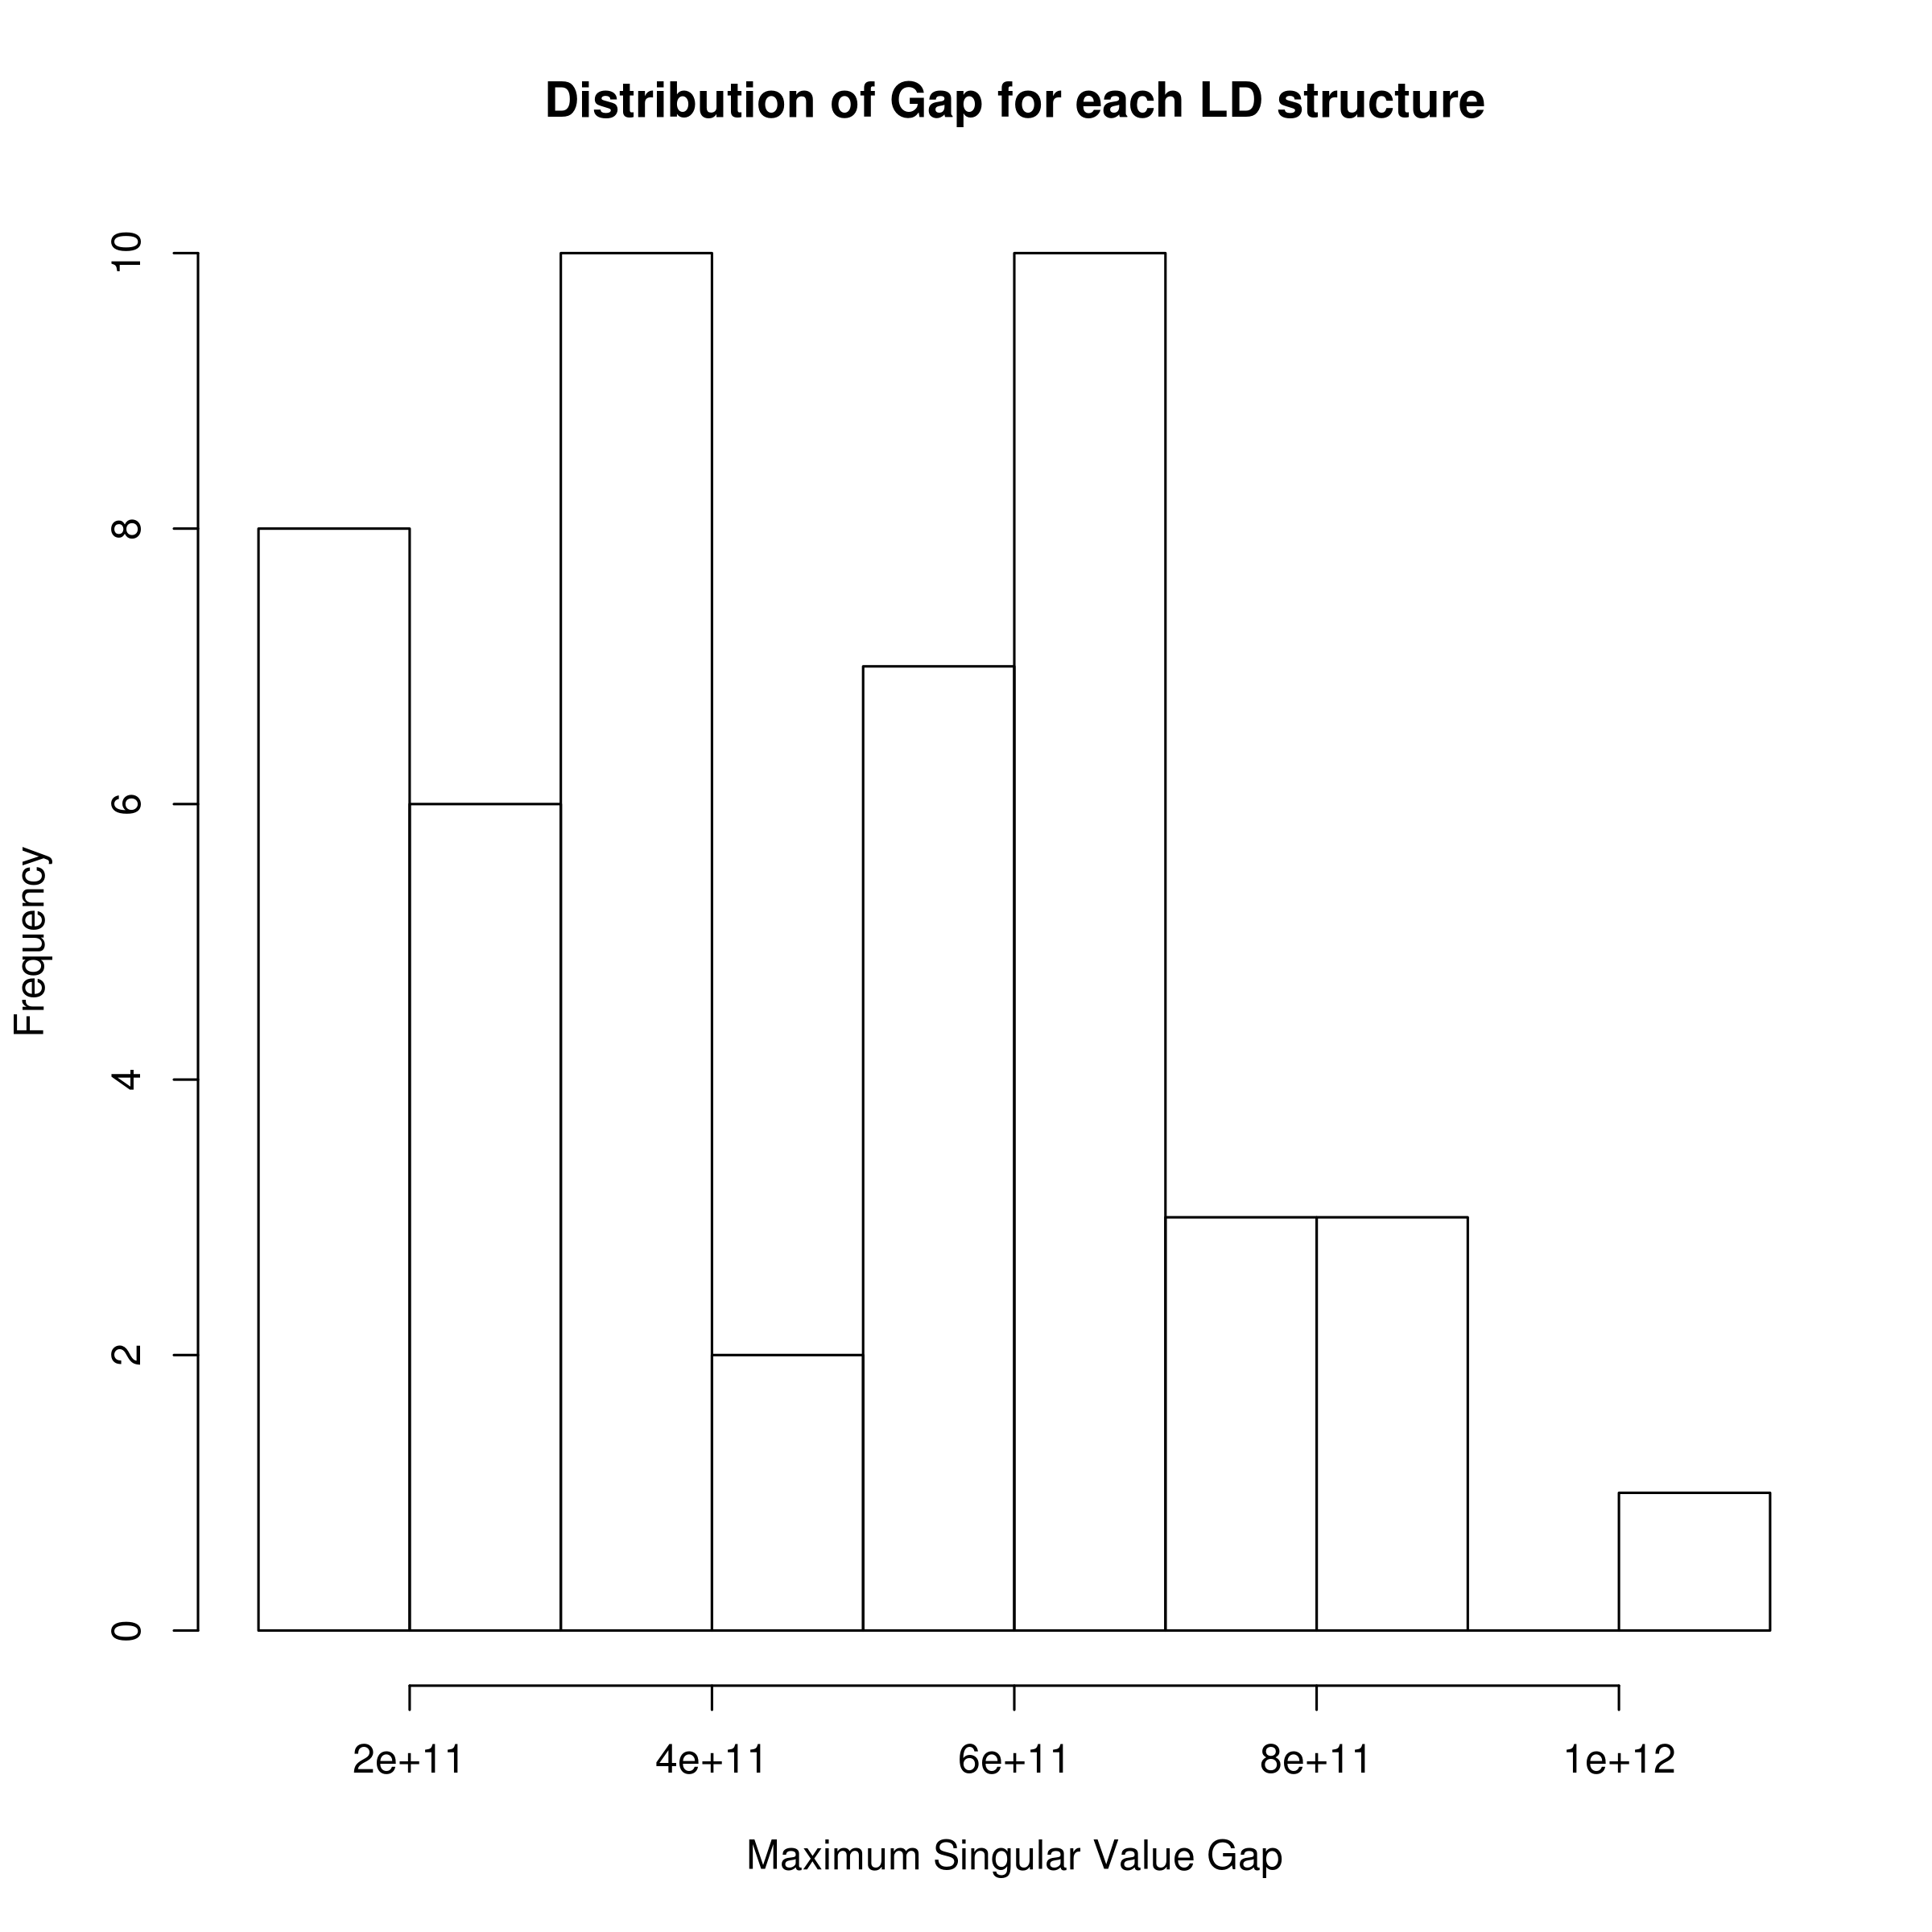
\includegraphics[width=0.5\textwidth]{figure/singular_value_distribution.png}
				\label{fig:singularValueDist}
			\end{figure}
			
			By employing the \gls{tSVD} as a method for regularization, we were able to solve the ill-posed \cref{eq:shrekEq}, and obtain the estimated heritability.
			
			
	
		\subsection{Extreme Phenotype Selections}
		%Explain why we perform extreme phenotype selections
		\cref{eq:fullShrek} can naturally be applied to the quantitative trait scenario. 
		%Explain how to apply the heritability estimation in the extreme phenotype situation
		\subsection{Case Control Studies}
	\section{Simulation}
		We implemented the heritability estimation in \gls{shrek} and in order to assess how well \gls{shrek} performs for heritability estimation in comparison to other current methods, we performed a series of systematic simulations.
		In these simulations, we compared the performance of \gls{shrek} with \gls{gcta}\citep{Yang2011} and the \gls{ldsc}\citep{Bulik-Sullivan2015} with and without the intercept estimation function (-{}-no-intercept). 
		
		Through simulation, we can obtain the sample distribution of the heritability estimate under different study designs (e.g. Quantitativat traits, Case-Control studies or extreme phenotype selection). 
		We can also evaluate the performance of different methods under varying genetic architecture (e.g. different number of Snps, different LD structures) or even with different disease models (e.g. different number of causal Snps, different heritability).
		
		\subsection{Quantitative Trait}
			To model a polygenic quantitative trait in \gls{GWAS} and \gls{wgs} studies, we assigned per-\gls{SNP} effect sizes drawn from the exponential distribution with $\lambda = 1$ to varying number of causal variants $k$ and heritabilities $H$ where $H\in[0,1)$. 
			An exponential distribution was chose based on work of \citet{Orr1998} which suggested the exponential distribution provides a heuristic expectation about the genetic architecture of adaptation.
			
			To simulate samples with genetic architecture comparable to true human population, \textit{HAPGEN2}\citep{Su2011} was used.
			$n$ samples were simulated based on the genome structure of the \gls{CEU} with 20,000 SNPs where $k$ of those are causal.
			In order to simulate a quantitative trait with target heritability of $h$, the per SNPs effect were calculated as
			\begin{align}
			\beta_i &\sim exp(1)\notag\\
			\boldsymbol{\beta}&=(\beta_1,\beta_2,...,\beta_k)^t\notag\\
			\boldsymbol{\gamma} &= \frac{h}{k}\boldsymbol{\beta}\notag\\
			H&=\boldsymbol{1}^T\boldsymbol{\gamma}
			\label{eq:snpEffect}
			\end{align}
			where $\boldsymbol{\gamma}$ is the vector of per SNP effect size and $H$ is the simulated heritability.
			The only exception is when $k=1$ where $\beta = H$ such that we can simulate SNPs with large effect size.
			
			After the per \gls{SNP} effect were simulated, we distribute the effect size to $k$ randomly selected \gls{SNP}(s) according to their \gls{maf}.
			Therefore for \glspl{SNP} with a small \gls{maf}, a larger effect size is given such that the effect size distribution in our simulation will follow that observed in the real life scenario\citep{Manolio2009}.
			
			
			Assuming $\boldsymbol{X}$ to be the standardized genotype of $k$ causal SNPs in $n$ samples, one can get the phenotype of the simulated samples using
			\begin{align}
			\epsilon_i&\sim N(0,\sqrt{\mathrm{Var}(\boldsymbol{X\gamma})\frac{1-H}{H}} )\notag\\
			\boldsymbol{\epsilon} &= (\epsilon_1,\epsilon_2,...,\epsilon_n)^t\notag\\
			\boldsymbol{y} &= \boldsymbol{X\gamma}+\boldsymbol{\epsilon}
			\label{eq:simulationOfPhenotype}
			\end{align}
			
			For each batch of simulated samples, we calculate the estimated heritability using \gls{shrek}, \gls{gcta}, \gls{ldsc} without intercept estimation and \gls{ldsc} with intercept estimate (\textit{\texorpdfstring{LDSC\textsubscript{In}}}) for each $H$.
			In each iteration, the sample genotype was provided to \gls{gcta} for the calculation of genetic relationship matrix (GRM) whereas for \gls{shrek} and \gls{ldsc} 500 additional samples were simulated based on the 1000 genome project \gls{CEU}\parencite{Project2012} to construct the \gls{LD} matrix and calculate the \gls{LD} score respectively.   
			The whole process were repeated 100 times to obtain the empirical variance of the estimates,.
			In each iteration, new set of samples were simulated with the \glspl{SNP} set, the causal \glspl{SNP} and the per \gls{SNP} effect size remain unchanged for each $H$.
			
			In order to determine a realistic and reasonable sample size for all simulation condition, we manually curated the sample size of all the studies presented on the \gls{GWAS} Catalog\cite{Welter2014} (version 2015-07-17) to get the distribution of sample size in existing studies.
			It was observed that the mean sample size of all published \gls{GWAS} is $\sim$ 7,200 samples. 
			Thus, we consider a simulation sample size of 7,200 should be comparable to general \gls{GWAS} studies.
			Although a large sample size are generally required for \gls{GWAS}, it might also worthwhile for one to test the performance when only small sample size is available.
			If the tools perform well with a small sample size, it will be beneficial to studies of rare complex traits where it is often difficult to collect a large amount of samples.
			As a result of that, we also perform simulation with 1,000 samples.
			
			Another consideration is the number of causal \glspl{SNP} as it determine the complexity of the trait which usually directly proportional with the number of causal \glspl{SNP}. 
			To capture the full spectrum of trait complexity (e.g. Mendelian to Oligogenic to Complex Traits), we selected number of causal \glspl{SNP} to be $k\in\{1,10,50,100,1000\}$ such that effect size$ \in(0,\frac{1}{k})$.To simplify the simulation procedure, all causal \glspl{SNP} were included within the data.
			
			To summarize, 
			\begin{enumerate}
				\item Randomly select 200,000 \glspl{SNP} from chromosome 1
				\item Randomly generate $k$ effect size following \cref{eq:snpEffect} where $k \in \{1,10,50,100,1000\}$
				\item Randomly assign the effect size to $k$ \glspl{SNP} where \glspl{SNP} with small \gls{maf} will get a large effect size.
				\item Simulate $n$ samples using \textit{HAPGEN2} with $n \in \{1000,7200\}$
				\item Repeat step 4 100 times
				\item Repeat step 1-5 50 times
			\end{enumerate}
		\subsection{Case Control Studies}
		Simulate of the case control studies are very much like that in the quantitative trait settings. 
		
		\subsection{Exreme Phenotype Selections}
	\section{Result}
		The heritabilibty estimation were implemented in \gls{shrek} and is available on \url{https://github.com/choishingwan/shrek}.
		
	\section{Discussion}
	
	\chapter{Heritability of Schizophrenia}
	\section{Introduction}
	\section{Heritability Estimation}
	This will be a very simple section, focused on how to perform the heritability estimation on \acrfull{SCZ}.
	Should also tokenize the heritability into subcategories (e.g. immune, neuron, etc)
	%Should not put too much weight into it, otherwise it will be a direct copy of LDSC. Won't really add much power. 
	\subsection{Methodology}
	\subsection{Result}
	\section{Brain development and Schizophrenia}
	Here we will perform the WGCNA and brain development network.
	Seeing how the whether if any brain development network were enriched with SNPs that explain the variance of phenotype
	%Instead, we should put most focus here as no one has done it before
	\subsection{Methodology}
	\subsection{Result}
	\section{Discussion}
	\chapter{Heritability of Response to antipsychotic treatment}
	\section{Introduction}
	Here we try to use Beatrice's data and estimate the heritability explained in drug response.
	Should also repeat the region-wise heritability
	\section{Methodology}
	\section{Result}
	\section{Discussion}
	\chapter{Risk Prediction}
	\section{Methodology}
	We can define the traditional \gls{PGS} as
	\begin{equation}
	\hat{Y} = diag(\beta)X
	\end{equation}
	where $X$ is the standardized genotype, $\beta$ is the test-statistic calculated from other studies. 
	
	
	\subsection{Simulation}
	\section{Result}
	\section{Discussion}
	\chapter{Conclusion}
	\backmatter
	\printbibliography
	\chapter*{Appendix}
\end{document}


